\documentclass[final]{beamer}
\mode<presentation>
{
 %\usetheme{Berlin}
 % \usetheme{Aachen}
%  \usetheme{Oldi6}
%  \usetheme{I6td}
 \usetheme{I6dv}
%  \usetheme{I6pd}
%  \usetheme{I6pd2}
}

\usepackage{bm}

\usepackage{times}
\usepackage{amsmath,amssymb,amsthm}

\usepackage[english]{babel}
\usepackage[latin1]{inputenc}

\usepackage{graphicx}
\usepackage{tabularx}
\usepackage{natbib}


\usepackage{hyperref,url}
\usepackage{amsmath,amssymb,amsthm}
\usepackage{tikz}
%\usepackage{float,subcaption,graphicx}
\usepackage{stmaryrd,wasysym,clrscode}
\usepackage{etex,etoolbox}
\usepackage{ifthen}
\usetikzlibrary{patterns,positioning}

%%% Added by Jonathan %%%
\def\[#1\]{\begin{align}#1\end{align}}
\def\(#1\){\begin{align*}#1\end{align*}}
\newcommand{\ip}[2]{\left\langle #1, #2 \right\rangle}
\definecolor{NAColor}{rgb}{.75,0,.75}
\newcommand{\NA}[1]{\textcolor{NAColor}{($\star$) #1}}
\newcommand{\dee}{\mathrm{d}}
\newcommand{\algname}[1]{\textsc{\lowercase{#1}}}
\def\argmax{\operatornamewithlimits{arg\,max}}
\def\argmin{\operatornamewithlimits{arg\,min}}
\newcommand{\defined}{\ensuremath{\triangleq}}
\newcommand{\bprf}{\begin{proof}}
\newcommand{\eprf}{\end{proof}}
\newcommand{\blem}{\begin{lemma}}
\newcommand{\elem}{\end{lemma}}
\newcommand{\eps}{\epsilon}
%%% End added by Jonathan %%%

\newcommand{\lc}[1]{#1_{\mathrm{loc}}}
\newcommand{\eq}[1]{\stackrel{\mathrm{#1}}{=}}
\DeclareMathOperator{\Var}{Var}
\DeclareMathOperator{\sign}{sign}
\DeclareMathOperator{\MMD}{MMD}
\newcommand{\MMDr}{\tilde{\MMD}}
\DeclareMathOperator{\Tr}{Tr}
\newcommand{\inner}[2]{\langle #1, #2 \rangle}
\newcommand{\E}{\mathcal{E}}
\newcommand{\eqdef}{\stackrel{\mathrm{def}}{=}}
\newcommand{\bP}{\mathbb{P}}
\newcommand{\bI}{\mathbb{I}}
\newcommand{\bE}{\mathbb{E}}
\newcommand{\sF}{\mathcal{F}}
\newcommand{\sH}{\mathcal{H}}
\newcommand{\sC}{\mathcal{C}}
\newcommand{\sM}{\mathcal{M}}
\newcommand{\sE}{\mathcal{E}}
\newcommand{\C}{\mathcal{C}}
\newcommand{\sB}{\mathcal{B}}
\newcommand{\bR}{\mathbb{R}}
\newcommand{\bN}{\mathbb{N}}
\newcommand{\bZ}{\mathbb{Z}}
\newcommand{\sI}{\mathcal{I}}
\newcommand{\sP}{\mathcal{P}}
\newcommand{\sX}{\mathcal{X}}
\newcommand{\sS}{\mathcal{S}}
\newcommand{\sJ}{\mathcal{J}}
\newcommand{\sR}{\mathcal{R}}
\newcommand{\sN}{\mathcal{N}}
\newcommand{\meet}{\wedge}
\newcommand{\RE}[2]{\operatorname{RE}\left(#1 \ \| \ #2\right)}
\newcommand{\KL}[2]{\operatorname{KL}\left(#1 \ \| \ #2\right)}
\newcommand{\KLm}[2]{\operatorname{KL}_m\left(#1 \ \| \ #2\right)}
\newcommand{\score}[2]{\operatorname{score}\left(#1 \ \| \ #2\right)}
\newcommand{\phih}{\hat{\phi}}
\newcommand{\psih}{\hat{\psi}}
\DeclareMathOperator{\supp}{supp}
\DeclareMathOperator{\loc}{loc}
\DeclareMathOperator{\lub}{lub}
\newcommand{\atom}[1]{#1^{\circ}}
\newcommand{\stitch}[2]{\overline{#1}^{#2}}
%\DeclareMathOperator{\argmin}{argmin}
%\DeclareMathOperator{\argmax}{argmax}

\newtheorem{theorem}{Theorem}[section]
\newtheorem{lemma}[theorem]{Lemma}
\newtheorem{proposition}[theorem]{Proposition}
\newtheorem{corollary}[theorem]{Corollary}
\newtheorem{assumption}[theorem]{Assumption}
\theoremstyle{definition}
\newtheorem{example}[theorem]{Example}
\newtheorem{definition}[theorem]{Definition}
\newtheorem{remark}[theorem]{Remark}
\newtheorem{property}[theorem]{Property}

\def\ci{\perp\!\!\!\perp}


%\usepackage[orientation=landscape,size=a0,scale=1.4]{beamerposter}
\usepackage[orientation=landscape,size=custom,width=121.92,height=91.44,scale=1.4]{beamerposter} % 48in x 36in

% Display a grid to help align images
%\beamertemplategridbackground[1cm]

\title%[] %(optional, use only with long paper titles)
{A Greedy Framework for First-Order Optimization}

%\subtitle {Include Only If Paper Has a Subtitle}

\author%[Author, Another] % (optional, use only with lots of authors)
{Jonathan Huggins$^{*1}$, Jacob Steinhardt$^{*2}$}

\institute[] % (optional, but mostly needed)
{$^{*}$Both authors contributed equally to this work. $^1$Massachusetts Institute of Technology. $^{2}$Stanford University.}

\date{December 2013}

\begin{document}

\begin{frame}{} 
%\titlepage  
%\vfill
\begin{columns}

%%%%%%%%%%%%%%%%%%%%%%%%%%%%%%%%%%%%%%%%%%%%%%%%%%
%%%% COLUMN 1		 						%%%%%%
%%%%%%%%%%%%%%%%%%%%%%%%%%%%%%%%%%%%%%%%%%%%%%%%%%
\begin{column}{0.46\linewidth}

%%%%%%%%%%%%%%%%%%%%%%%%%%%%%%
%%% BEGIN MOTIVATION BLOCK %%%
%%%%%%%%%%%%%%%%%%%%%%%%%%%%%%
\begin{block}{\large Motivation}
Suppose we want to solve the following \emph{saddle point} problem:
\[ \min_u \max_{\theta} L(u, \theta), \]
where $L(u,\theta) = h(u) + \langle u, \theta \rangle - R(\theta)$. 
We assume that $h$ and $R$ are both convex and that $\langle \cdot, \cdot \rangle$ 
is an arbitrary bilinear map.
\newline\newline
\textbf{Intuition:} $u$ is the ``primal'', $\theta$ is the ``dual''.
\newline\newline
\textbf{Tie-in with optimization:} can recast as minimizing
\[ L(u) \eqdef \max_{\theta} L(u, \theta) = h(u) + R^*(u). \]

Here $R^*(u) \eqdef \max_{\theta} u^T\theta - R(\theta)$ is the 
\emph{Fenchel conjugate} of $\theta$.
\end{block}

\begin{block}{\large Fenchel conjugate properties}
Fenchel conjugates are a key component of \emph{Legendre-Fenchel duality} 
and also show up in mirror descent. It turns out that they will also be 
important for generalizing the Frank-Wolfe algorithm.
\newline\newline
\textbf{Property 1:} If $R$ is convex then $R^{**} = R$.
\qquad\qquad
\textbf{Property 2:} $\partial R^*(u) = \argmin_{\theta} u^T\theta - R(\theta)$.
\end{block}
%%%%%%%%%%%%%%%%%%%%%%%%%%%%
%%% END MOTIVATION BLOCK %%%
%%%%%%%%%%%%%%%%%%%%%%%%%%%%

%%%%%%%%%%%%%%%%%%%%%%%%%%%%%%
%%% BEGIN TOO GREEDY BLOCK %%%
%%%%%%%%%%%%%%%%%%%%%%%%%%%%%%
\begin{block}{\large Being (Too) Greedy}
\begin{columns}[t]
\begin{column}{.48\linewidth}
We might try the following ``iterative best response'' updates:
\begin{align*}
u_t\,\,\,\,\,\, &= \argmin_{u} L(u,\theta_t) \\
\theta_{t+1}   &= \argmax_{\theta} L(u_t, \theta)
\end{align*}
\end{column}
\begin{column}{.48\linewidth}
{\bf Problem:} let $u,\theta \in \bR$, $h(u) = \frac{1}{2}u^2$, $R(\theta) = \frac{1}{2}\theta^2$. 
Then:
\begin{align*}
u_t\,\,\,\,\,\, &= \argmin_u \left[\frac{1}{2}u^2 + u\theta\right]             = -\theta_t \\
\theta_{t+1}    &= \argmax_{\theta} \left[u\theta - \frac{1}{2}\theta^2\right] = u_t
\end{align*}
\begin{center}
\textcolor{red}{OSCILLATION}
\end{center}
\end{column}
\end{columns}
\end{block}
%%%%%%%%%%%%%%%%%%%%%%%%%%%%
%%% END TOO GREEDY BLOCK %%%
%%%%%%%%%%%%%%%%%%%%%%%%%%%%

%%%%%%%%%%%%%%%%%%%%%%%%%%%%%
%%% BEGIN ALGORITHM BLOCK %%%
%%%%%%%%%%%%%%%%%%%%%%%%%%%%%
\begin{columns}[t]
\begin{column}{.43\linewidth}
\begin{block}{\large Being (Less) Greedy: \\ Boosted Mirror Descent}
Replace $u_t$ with a weighted average
\begin{align*}
\hat{u}_t &\eqdef \frac{1}{A_{t}} \sum_{s=1}^t \alpha_{s} u_s & A_{t} = \sum_{s=1}^{t} \alpha_{s}
\end{align*}
New updates (``dual'' algorithm):
\begin{align*}
u_t\,\,\,\,\,\, &= \argmin_{u} L(u,\theta_t)  = && \partial h^{*}(-\theta_{t}) \\
\theta_{t+1}    &= \argmax_{\theta} L(\hat{u}_t, \theta)  = &&\partial R^{*}(\hat u_{t})
\end{align*}
Alternatively, replace $\theta_{t}$ with a weighted average (``primal'' algorithm):
\begin{align*}
u_t\,\,\,\,\,\, &= \argmin_{u} L(u,\hat\theta_t) = && \partial h^{*}(-\hat\theta_{t}) \\
\theta_{t+1}    &= \argmax_{\theta} L(u_t, \theta) = &&\partial R^{*}(u_{t})
\end{align*}
\end{block}
\end{column}
\begin{column}{.53\linewidth}
\begin{block}{\large A Geometric Picture (Primal)}
\begin{center}
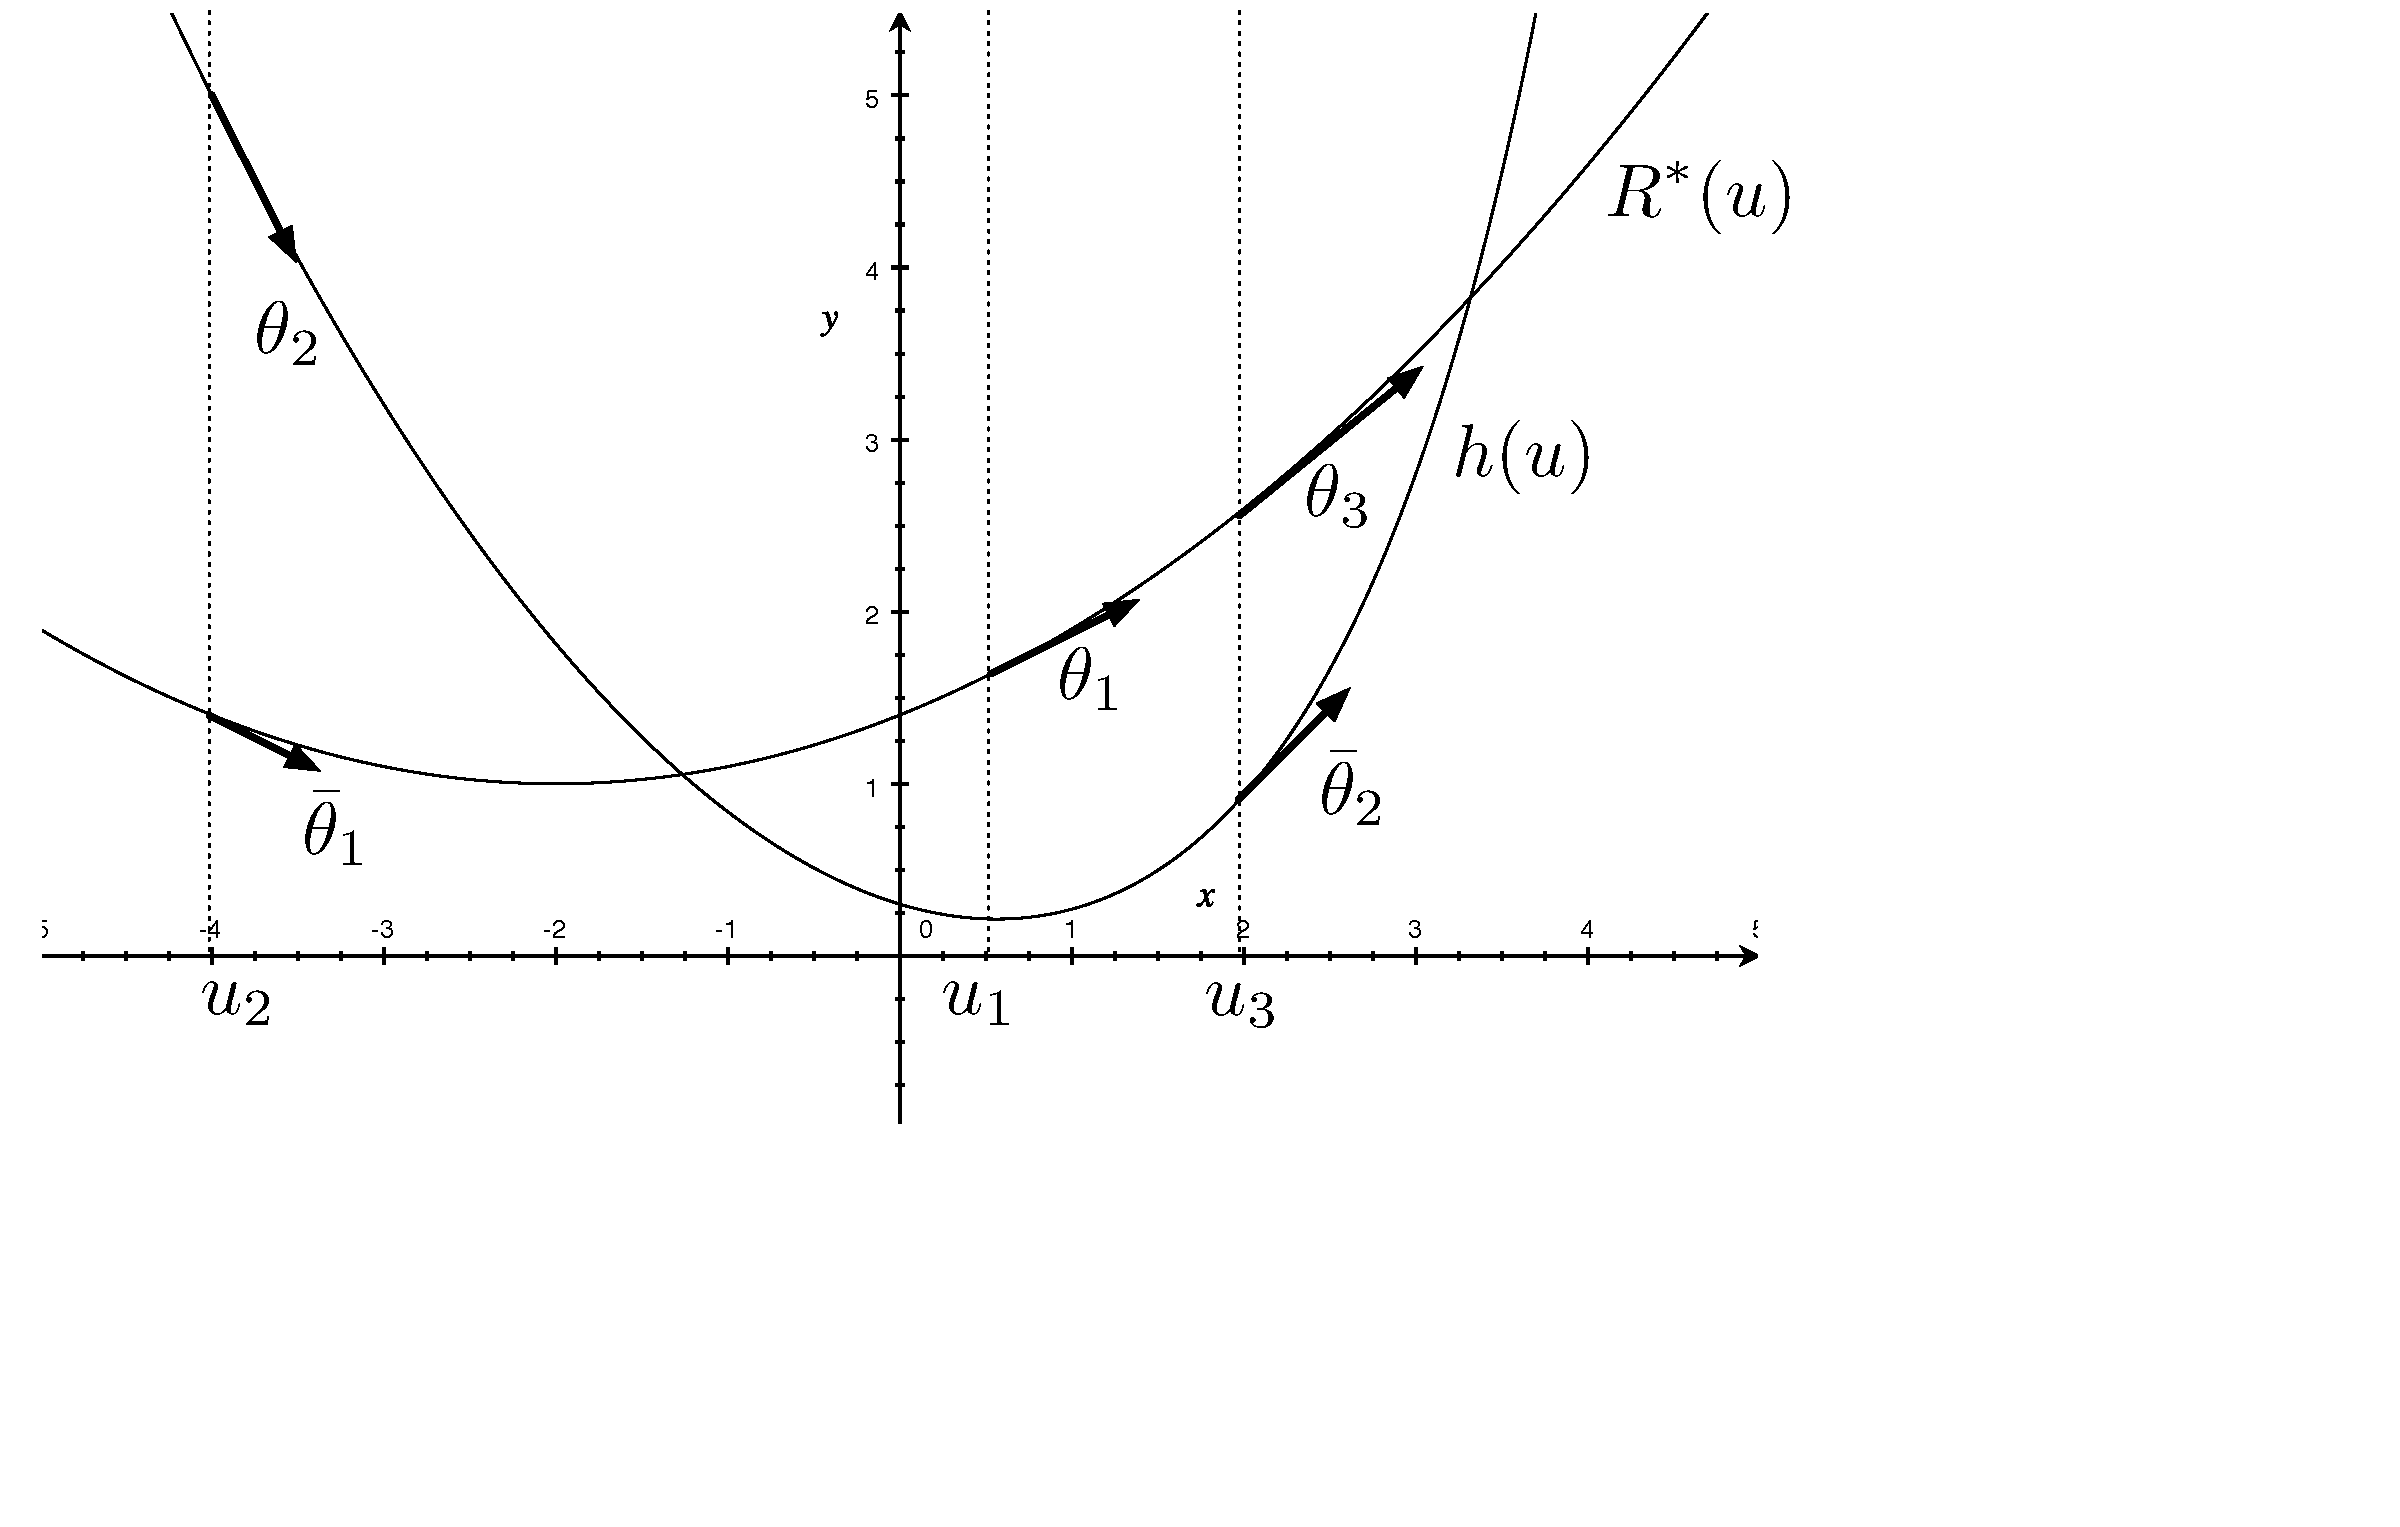
\includegraphics[width=10in]{figures/primal-demo.pdf}
\end{center}
For the primal algorithm,
\begin{align*}
u_t\,\,\,\,\,\, &= \partial h^{*}(-\hat\theta_{t}) \text{ is a point where $-\hat\theta_{t} \in \partial h$} \\ 
\theta_{t+1}    &= \partial R^{*}(u_{t}) \text{ is the gradient of $R^{*}$ at $u_{t}$}
\end{align*}
So $u_{t}$ is chosen such that the gradient contributed by $h$ at $u_{t}$ cancels out the gradient contributed by $R^{*}$. 
\end{block}
\end{column}
\end{columns}
%%%%%%%%%%%%%%%%%%%%%%%%%%%
%%% END ALGORITHM BLOCK %%%
%%%%%%%%%%%%%%%%%%%%%%%%%%%
\end{column}	

	

%%%%%%%%%%%%%%%%%%%%%%%%%%%%%%%%%%%%%%%%%%%%%%%%%%
%%%% COLUMN 2		 						%%%%%%
%%%%%%%%%%%%%%%%%%%%%%%%%%%%%%%%%%%%%%%%%%%%%%%%%%
\begin{column}{0.50\linewidth}

%%%%%%%%%%%%%%%%%%%%%%%%%%%%%%%%
%%% BEGIN APPLICATIONS BLOCK %%%
%%%%%%%%%%%%%%%%%%%%%%%%%%%%%%%%
\begin{block}{\large Special Cases and Applications}
Many particular algorithms can be cast into our framework.
\begin{columns}[t]
\begin{column}{0.01\linewidth}\end{column}
\begin{column}{0.47\linewidth}

\begin{block}{Conditional gradient (Frank-Wolfe)}
Let $h \equiv 0$. Then we have the updates
\begin{align*}
u_t &= \argmin_u u^T\theta_t \\
 &= \argmin_u u^T\partial R^*(\hat{u}_{t-1}),
\end{align*}
which is the Frank-Wolfe update for $R^*$.
\end{block}

\begin{block}{Thresholded Frank-Wolfe}
Suppose we want to minimize $\|u\|_1 + R^*(u)$. Then 
we can consider the following 
\emph{thresholded Frank-Wolfe algorithm}:
\begin{align*}
u_t &= \argmin_u \|u\|_1 + u^T\partial R^*(\hat{u}_{t-1}),
\end{align*}
which converges at the same rate as conditional gradient 
but also imposes sparsity.
\end{block}

\begin{block}{(Modified) subgradient}
Let $h(u) = \frac{\gamma}{2} \|u\|_2^2$. Then the primal version of the 
algorithm gives the updates:
\begin{align*}
u_{t+1} &= \argmin_{\theta} \frac{\gamma}{2}\|u\|_2^2 + u^T\hat{\theta}_t \\
 &= -\frac{1}{\gamma}\hat{\theta}_t \\
 &= -\frac{1}{\gamma} \frac{\sum_{s=1}^t \alpha_s \partial R^*(u_s)}{\sum_{s=1}^t \alpha_s}.
\end{align*}
\end{block}

\end{column}
\begin{column}{0.47\linewidth}
\begin{block}{AHK low-rank SDP solver}
Suppose we want to solve the SDP
\begin{align*}
\text{maximize }   & \Tr(A^TX) \\
\text{subject to } & X \succeq 0 \\
                  & X_{ii} \leq 1 \, \forall i
\end{align*}
Set \small{$L(X,y) = \Tr(A^TX) + \sum_{i=1}^n \left[y_i(X_{ii}-1) - \eta y_i\log y_i\right]$}.
Then updating $X$ is an eigenvalue problem and each update is rank $1$. This 
yields a variant of the Arora-Hazan-Kale fast SDP solver.
\end{block}

\begin{block}{$q$-herding}
The \emph{herding} algorithm finds a distribution $\mu$ over 
$\sX$ such that $\bE_{x \sim \mu}[\phi(x)] \approx \bar{\phi}$ 
for a given collection of moments $\phi$. It is equivalent to 
the dual version of our algorithm for
\[ L(\mu,\theta) = \bE_{x \sim \mu}\left[\theta^T[\phi(x)-\bar{\phi}]\right] - \frac{1}{2}\|\theta\|_2^2, \]
which hinges upon $\|\bar{\phi}\|_2$ existing. In infinite 
dimensions this may not be the case and we can instead use the 
\emph{$q$-herding} algorithm based on the updates
\[ L(\mu,\theta) = \bE_{x \sim \mu}\left[\theta^T[\phi(x)-\bar{\phi}]\right] - \frac{1}{q}\|\theta\|_q^q, \]
which only requires that $\|\bar{\phi}\|_p$ exists, where $\frac{1}{p} + \frac{1}{q} = 1$.
\end{block}

\end{column}
\end{columns}
\end{block}
%%%%%%%%%%%%%%%%%%%%%%%%%%%%%%
%%% END APPLICATIONS BLOCK %%%
%%%%%%%%%%%%%%%%%%%%%%%%%%%%%%

%%%%%%%%%%%%%%%%%%%%%%%%%%%%%%%
%%% BEGIN CONVERGENCE BLOCK %%%
%%%%%%%%%%%%%%%%%%%%%%%%%%%%%%%
\begin{block}{\large Convergence of Boosted Mirror Descent}
\begin{columns}[t]
\begin{column}{0.01\linewidth}\end{column}
\begin{column}{0.47\linewidth}
\begin{theorem}
Consider the primal (respectively the dual) algorithm. Suppose that $h$ ($R$) is strongly convex with respect to a norm $\|\cdot\|$ 
and let $r = \sup_{\theta} \|\theta\|_{*}$ ($r = \sup_{u} \|u\|_{*}$). Then
\[ \sup_{\theta} L(\hat{u}, \theta) \leq \sup_{\theta} L(u^*, \theta) + \frac{2r^2}{A_T} \sum_{t=1}^T \frac{\alpha_{t+1}^2A_t}{A_{t+1}^2}. \]
\end{theorem}
\end{column}
\begin{column}{0.47\linewidth}
\begin{corollary} 
Under the hypotheses of the Theorem, for $\alpha_{t} = 1$ we have
\[ \sup_{\theta} L(\hat{u}, \theta) \leq \sup_{\theta} L(u^*, \theta) + \frac{2r^2 (\log (T) + 1)}{T}. \]
and for $\alpha_t = t$ we have
\[ \sup_{\theta} L(\hat{u}, \theta) \leq \sup_{\theta} L(u^*, \theta) + \frac{8r^2}{T}. \]
\end{corollary}
\end{column}
\end{columns}
\end{block}
%%%%%%%%%%%%%%%%%%%%%%%%%%%%%
%%% END CONVERGENCE BLOCK %%%
%%%%%%%%%%%%%%%%%%%%%%%%%%%%%

%%%%%%%%%%%%%%%%%%%%%%%%%%%%%%%%%%%%
%%%% BEGIN AHK APPLICATION BLOCK %%%
%%%%%%%%%%%%%%%%%%%%%%%%%%%%%%%%%%%%
%\begin{block}{\large Application: Solving SDPs}
%
%
%\end{block}
%%%%%%%%%%%%%%%%%%%%%%%%%%%%%%%%%%
%%%% END AHK APPLICATION BLOCK %%%
%%%%%%%%%%%%%%%%%%%%%%%%%%%%%%%%%%
%
%%%%%%%%%%%%%%%%%%%%%%%%%%%%%%%%%%%%%%%%%%
%%%% BEGIN Q-HERDING APPLICATION BLOCK %%%
%%%%%%%%%%%%%%%%%%%%%%%%%%%%%%%%%%%%%%%%%%
%\begin{block}{\large Application: $q$-herding}
%
%
%\end{block}
%%%%%%%%%%%%%%%%%%%%%%%%%%%%%%%%%%%%%%%%
%%%% END Q-HERDING APPLICATION BLOCK %%%
%%%%%%%%%%%%%%%%%%%%%%%%%%%%%%%%%%%%%%%%

%%%%%%%%%%%%%%%%%%%%%%%%%%%%%%%%%%%
%%% BEGIN ACKNOWLEDGMENTS BLOCK %%%
%%%%%%%%%%%%%%%%%%%%%%%%%%%%%%%%%%%
\begin{block}{\small Acknowledgements}
{\tiny Thanks to Cameron Freer, Simon Lacoste-Julien, Martin Jaggi, Percy Liang, Arun Chaganty, and Sida Wang 
for helpful discussions. JS was supported by the Hertz Foundation. JHH was supported by the U.S. Government under FA9550-11-C-0028 and awarded by the Department of Defense, Air Force Office of Scientific Research, National Defense Science and Engineering Graduate (NDSEG) Fellowship, 32 CFR 168a.}
\end{block}
%%%%%%%%%%%%%%%%%%%%%%%%%%%%%%%%%
%%% END ACKNOWLEDGMENTS BLOCK %%%
%%%%%%%%%%%%%%%%%%%%%%%%%%%%%%%%%

%%%%%%%%%%%%%%%%%%%%%%%%%%%%%%%%%
%%%% BEGIN BIBLIOGRAPHY BLOCK %%%
%%%%%%%%%%%%%%%%%%%%%%%%%%%%%%%%%
%\begin{block}{\small References}
%\begin{footnotesize}
%\bibliographystyle{plainnat}
%\bibliography{herding}
%\end{footnotesize}
%\end{block}
%%%%%%%%%%%%%%%%%%%%%%%%%%%%%%%
%%%% END BIBLIOGRAPHY BLOCK %%%
%%%%%%%%%%%%%%%%%%%%%%%%%%%%%%%


\end{column}

\end{columns}
\end{frame}
\end{document}
